\paragraph{nonnative-mul}

\subparagraph{Target}
Check the multiplication relation among three nonnative target objects.

\subparagraph{Constraints logic}
\begin{itemize}
    \item Check equation for gadget: \verb|a * b = prod + modular * overflow|;
    \item Check that ``overflow.limb is U32'';
    \item Check that ``prod.limb is U32''.
\end{itemize}

\subparagraph{Process layout}
See \figref{fig:nonnative-mul-layout}.
\begin{figure}[!ht]
    \centering
    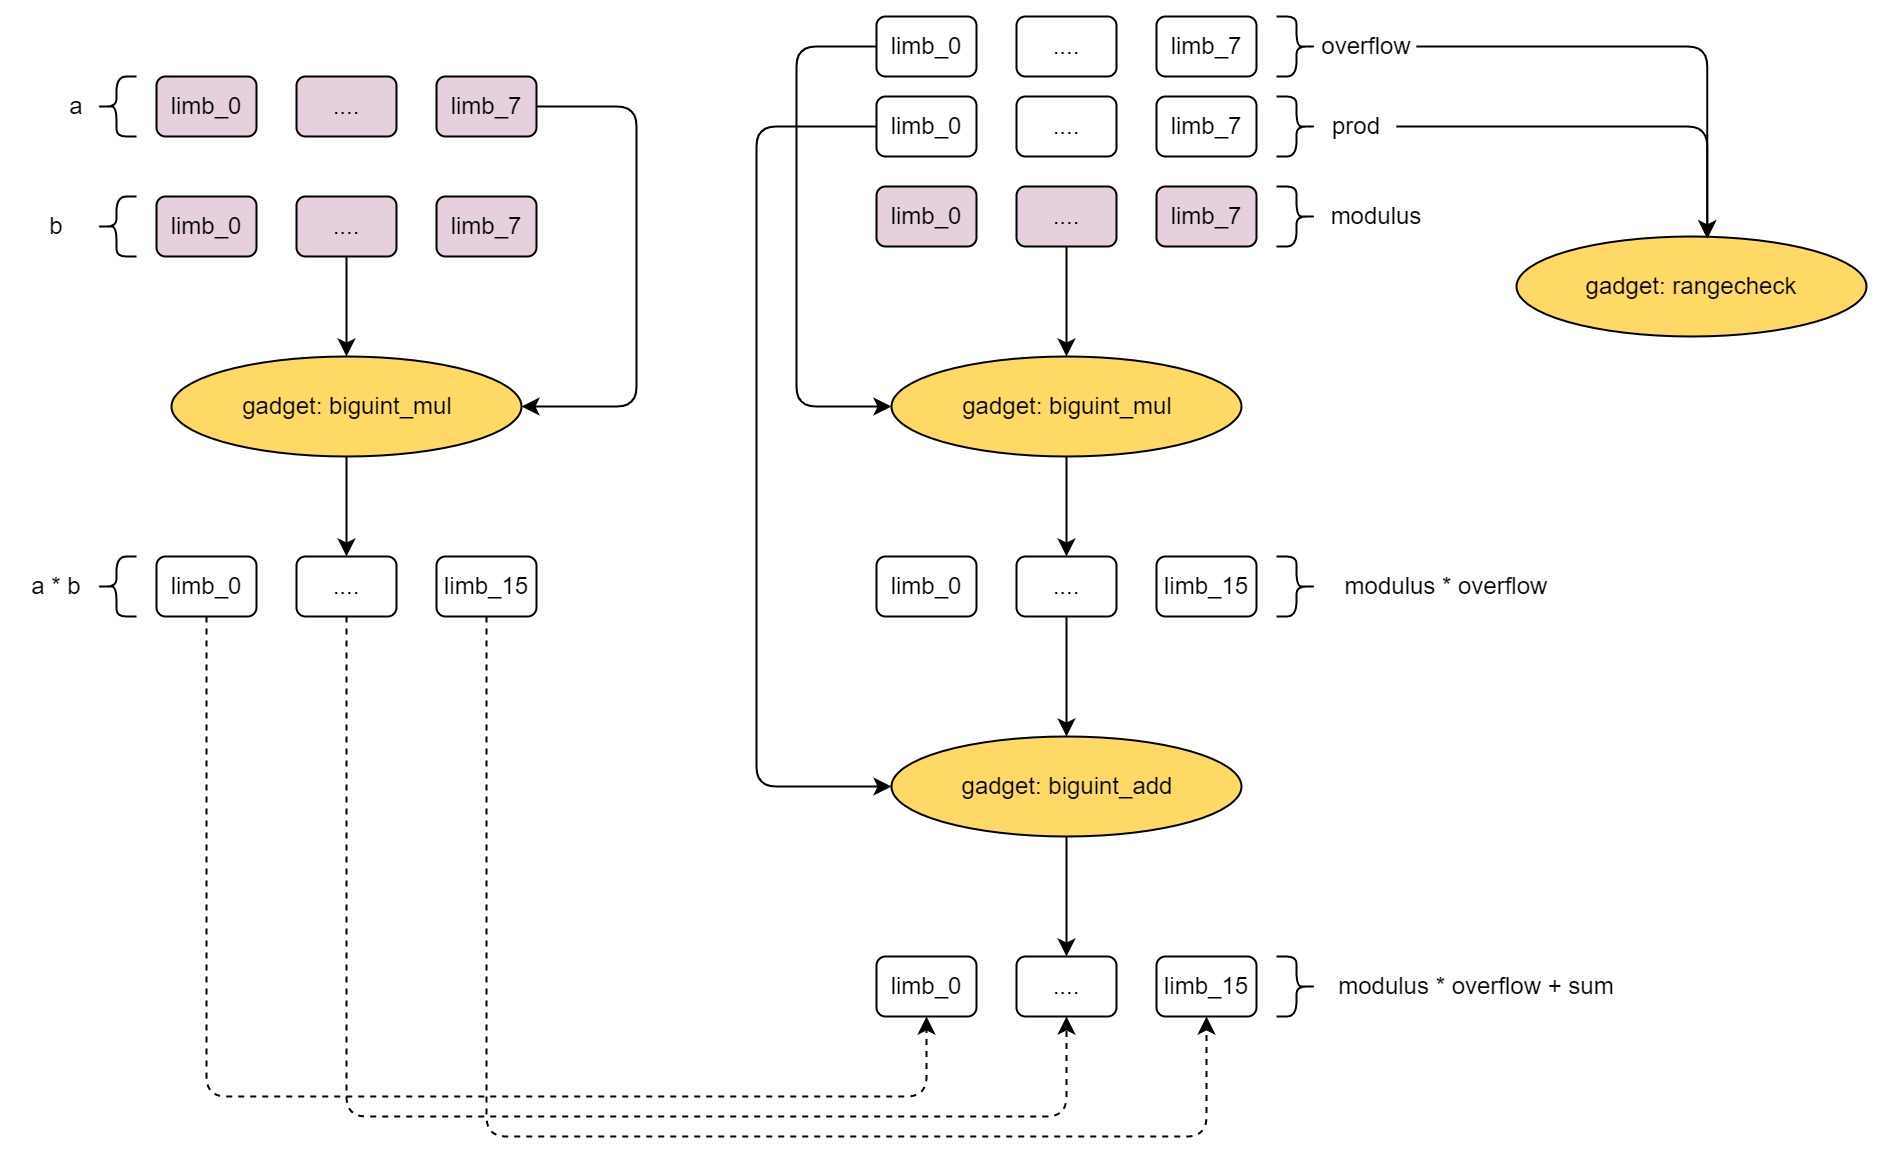
\includegraphics[width=0.8\textwidth]{nonnative-mul-layout.jpg}
    \caption{nonnative-mul layout}
    \label{fig:nonnative-mul-layout}
\end{figure}

\subparagraph{Constraints info and costs}
\begin{itemize}
    \item gadget biguint-add num: 1
    \item gadget biguint-mul num: 2
    \item gadget u32rangecheck num: 2
    \item gate type num: 9 = 7(U32AddManyGate\{3,5,7,9,11,13,15\}) + 1(U32RangeCheckGate) + 1(U32ArithmeticGate)
    \item gate instance num: 37 = 2(u32rangecheck) + 8(biguint-mul: constant-input) + 22(biguint-mul) + 1 + 3(biguint-add)
    \item copy-constraints: 583 = 8 * 2(u32rangecheck) + 3 * 3 + (4 + 6 + 8 + 10 + 12 + 14 + 16) * 4 + (8 * 8) * 3 + 17 * 4 + 18
\end{itemize}
